\documentclass{article}
\usepackage{Sweave, graphicx}
\begin{document}
\Sconcordance{concordance:05-results.tex:05-results.Rnw:%
1 22 1 51 0 1 21 16 1 8 0 19 1 6 0 28 1 4 0 18 1 4 0 5 1 4 0 6 1 4 %
0 2 1}

\title{The Title}
\author{A. Author}
\date{\today}
\maketitle




\section{Results}

\subsection{Modelling}
After forming the aforementioned regression models we found 10 coefficients that represent the best fit for each model. The resulting predictive function looks like:

\begin{equation}
Y = \beta_0 + \beta_1 X_1 + \beta_2 X_2 + \beta_3 X_3 + \beta_4 X_4 + \beta_5 X_5 + \beta_6 X_6 + \beta_7 X_7 + \beta_8 X_8 + \beta_9 X_9 + \beta_{10} X_{10} + \beta_{11} X_{11}
\end{equation}


\begin{center}
\begin{table}[ht]
\centering
\caption{Information about Model Coefficients} 
\begin{tabular}{rlrrr}
  \hline
 & Variables & Ridge & Lasso & PCR \\ 
  \hline
1 & UNEMP\_RATE & 0.000 & 0.000 & 0.000 \\ 
  2 & INEXPFTE & 0.000 & -0.000 & -0.008 \\ 
  3 & TUITIONFEE\_IN & -0.963 & -0.156 & -0.182 \\ 
  4 & AVGFACSAL & -0.786 & -0.067 & -0.089 \\ 
  5 & C150\_4 & -0.695 & -0.119 & -0.123 \\ 
  6 & C150\_L4 & 0.594 & 0.000 & 0.002 \\ 
  7 & RET\_FT4 & 0.978 & 0.000 & 0.027 \\ 
  8 & PELL\_COMP\_ORIG\_YR2\_RT & -2.752 & 0.000 & -0.111 \\ 
  9 & PELL\_COMP\_ORIG\_YR3\_RT & 0.491 & 0.042 & 0.125 \\ 
  10 & PELL\_COMP\_ORIG\_YR4\_RT & 1.372 & 0.000 & 0.020 \\ 
  11 & CDR2 & 0.498 & 0.120 & 0.166 \\ 
   \hline
\end{tabular}
\end{table}\end{center}

This table presents the fit between the prediction variables and the response variable ($Unemployment$) determined from the $cv.glmnet()$ and $pcr()$ functions, for each of our 3 models (Ridge, Lasso, PCR).

After finding the 5 predictive functions, we found the MSE's for each model:

\begin{center}

\begin{table}[ht]
\centering
\caption{Information about Mean Squared Errors} 
\begin{tabular}{rlr}
  \hline
 & Model & MSE \\ 
  \hline
1 & Ridge & 0.186 \\ 
  2 & Short Ridge & 12.797 \\ 
  3 & Lasso & 0.195 \\ 
  4 & Short Lasso & 17.114 \\ 
  5 & PCR & 0.271 \\ 
  6 & Short PCR & 1.446 \\ 
   \hline
\end{tabular}
\end{table}
\end{center}


Analysis of these numbers will reveal which model has the most predictive power.

\subsection{Hypothesis Testing}

For hypothesis testing method unemployment rate was set as our response variable and school funding was set as the independent variable (percent of students recieving financial aid).

If the amount of funding received by the school has no effect on quality of education rate, we should see little difference in the response variable (unemployment rate), and that difference is solely due to chance.

\graphicspath{ {../../images/} }
\begin{figure}
\centering
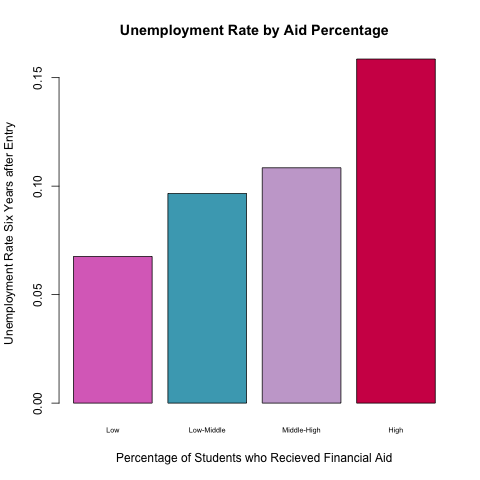
\includegraphics[scale=.5]{unemployment}
\caption{The}
\end{figure}


We looked for estimate (of effect of spending on unemployment). This value will reveal the relationship between our two variables.  A higher estimate means that spending has a significant effect on unemployment and a negative estimate means that spending has an inverse effect on unemployment

\begin{Schunk}
\begin{Soutput}
[1] NaN
\end{Soutput}
\end{Schunk}



\end{document}
